\documentclass[a4paper,11pt]{article}
\usepackage[margin=10mm]{geometry}
\usepackage{tikz}
\usepackage{helvet}
\renewcommand{\familydefault}{\sfdefault}
\pagestyle{empty}
\setlength{\parindent}{0pt}
\begin{document}
{\Large\bfseries LEFT TURN TEST}\par
\vspace{2mm}
{\small Black line width: 20 mm. Print at 100\% scale; disable fit-to-page scaling.}\par
\begin{center}
  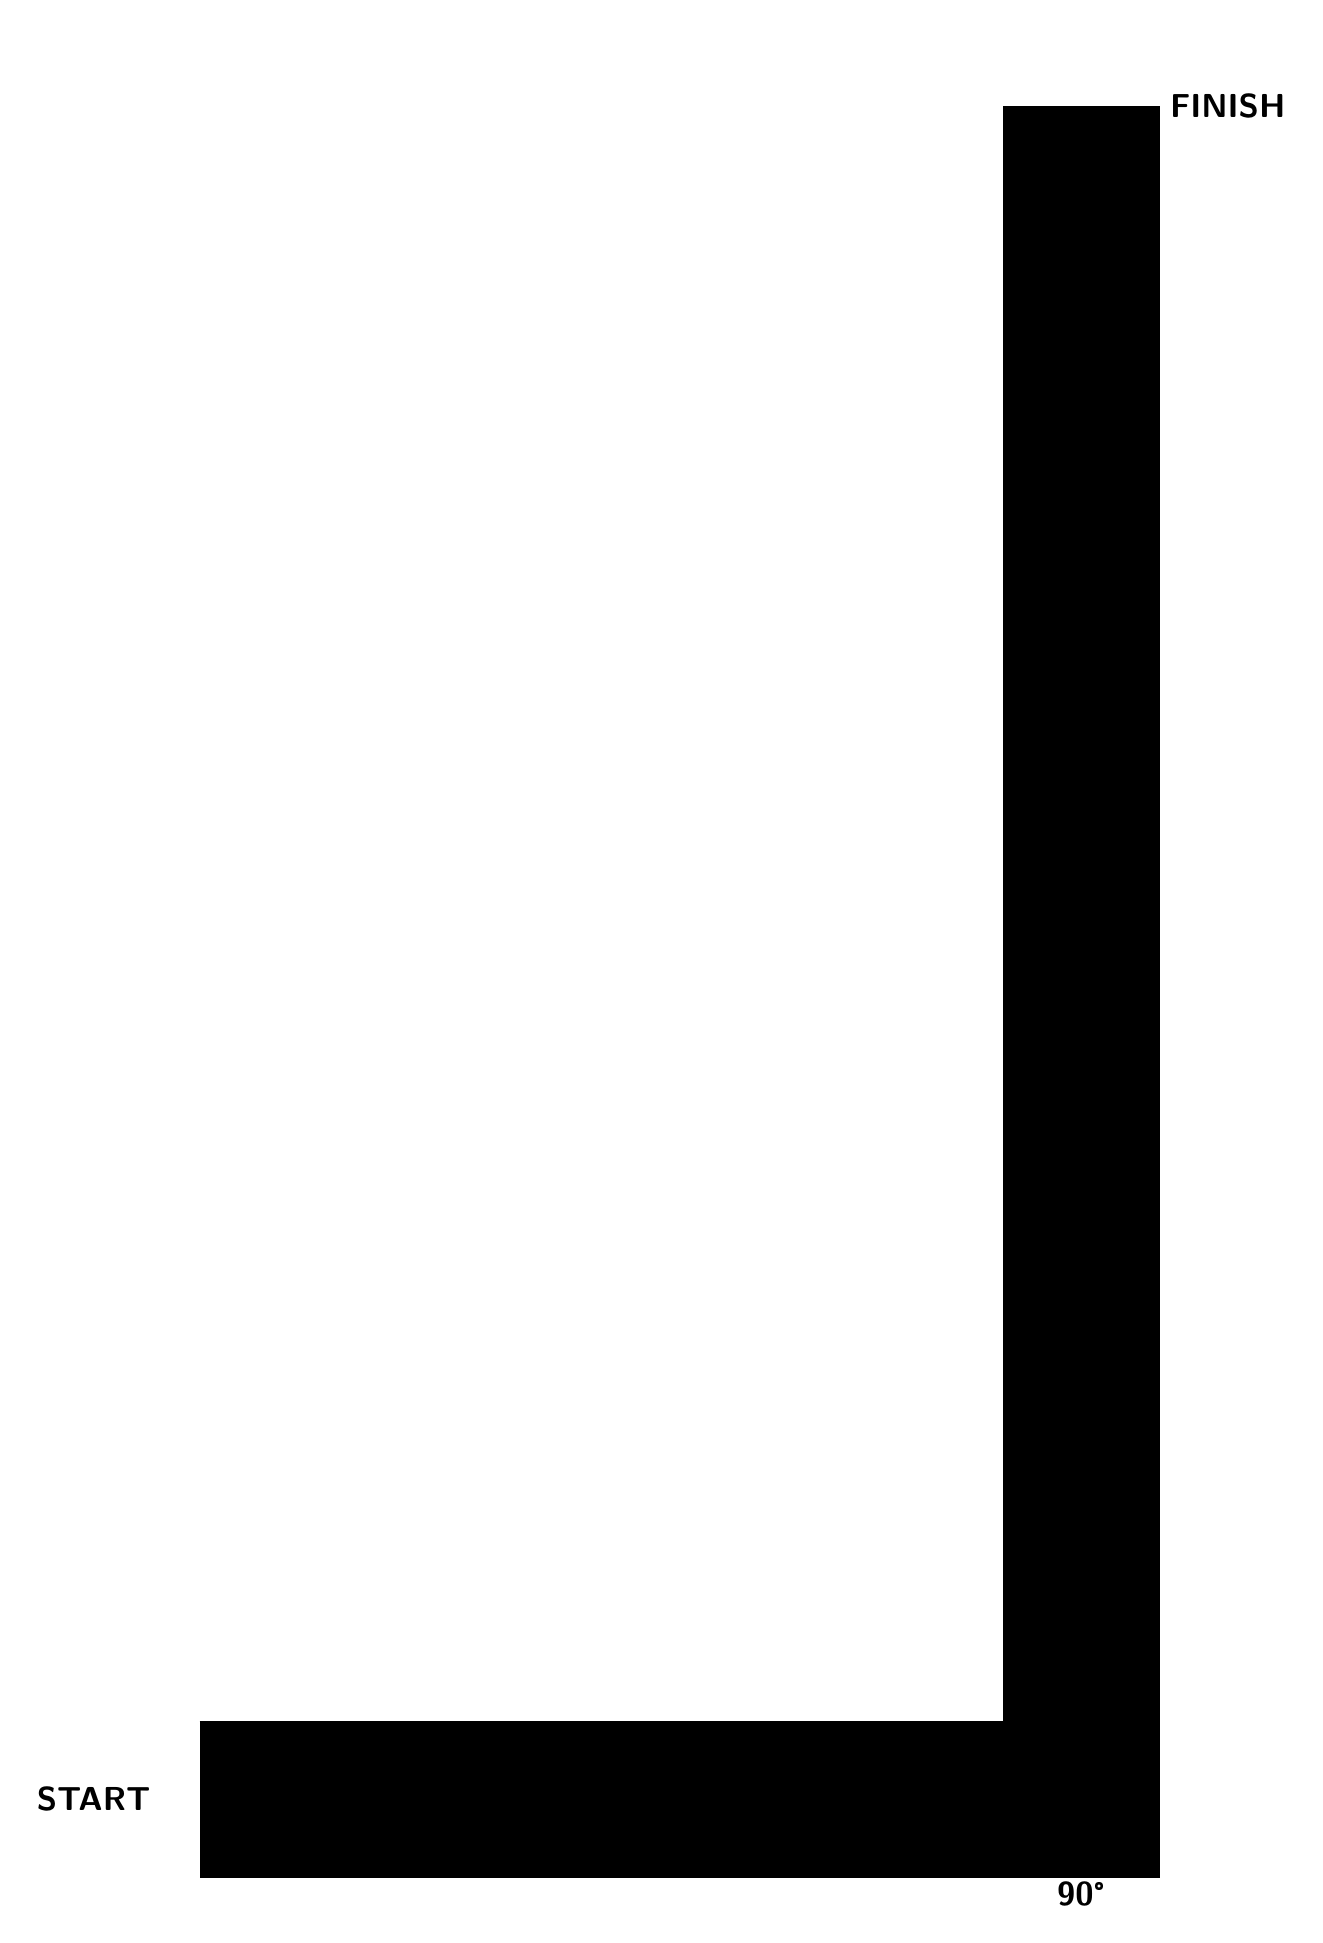
\begin{tikzpicture}[x=1mm,y=1mm]
    \draw[line width=20mm, black, line cap=butt] (18,30) -- (130,30) -- (130,245);
    \node[anchor=east, font=\large\bfseries] at (13,30) {START};
    \node[anchor=west, font=\large\bfseries] at (140,245) {FINISH};
    \node[font=\large\bfseries] at (130,18) {90\textdegree};
  \end{tikzpicture}
\end{center}

\newpage

{\Large\bfseries RIGHT TURN TEST}\par
\vspace{2mm}
{\small Black line width: 20 mm. Print at 100\% scale; disable fit-to-page scaling.}\par
\begin{center}
  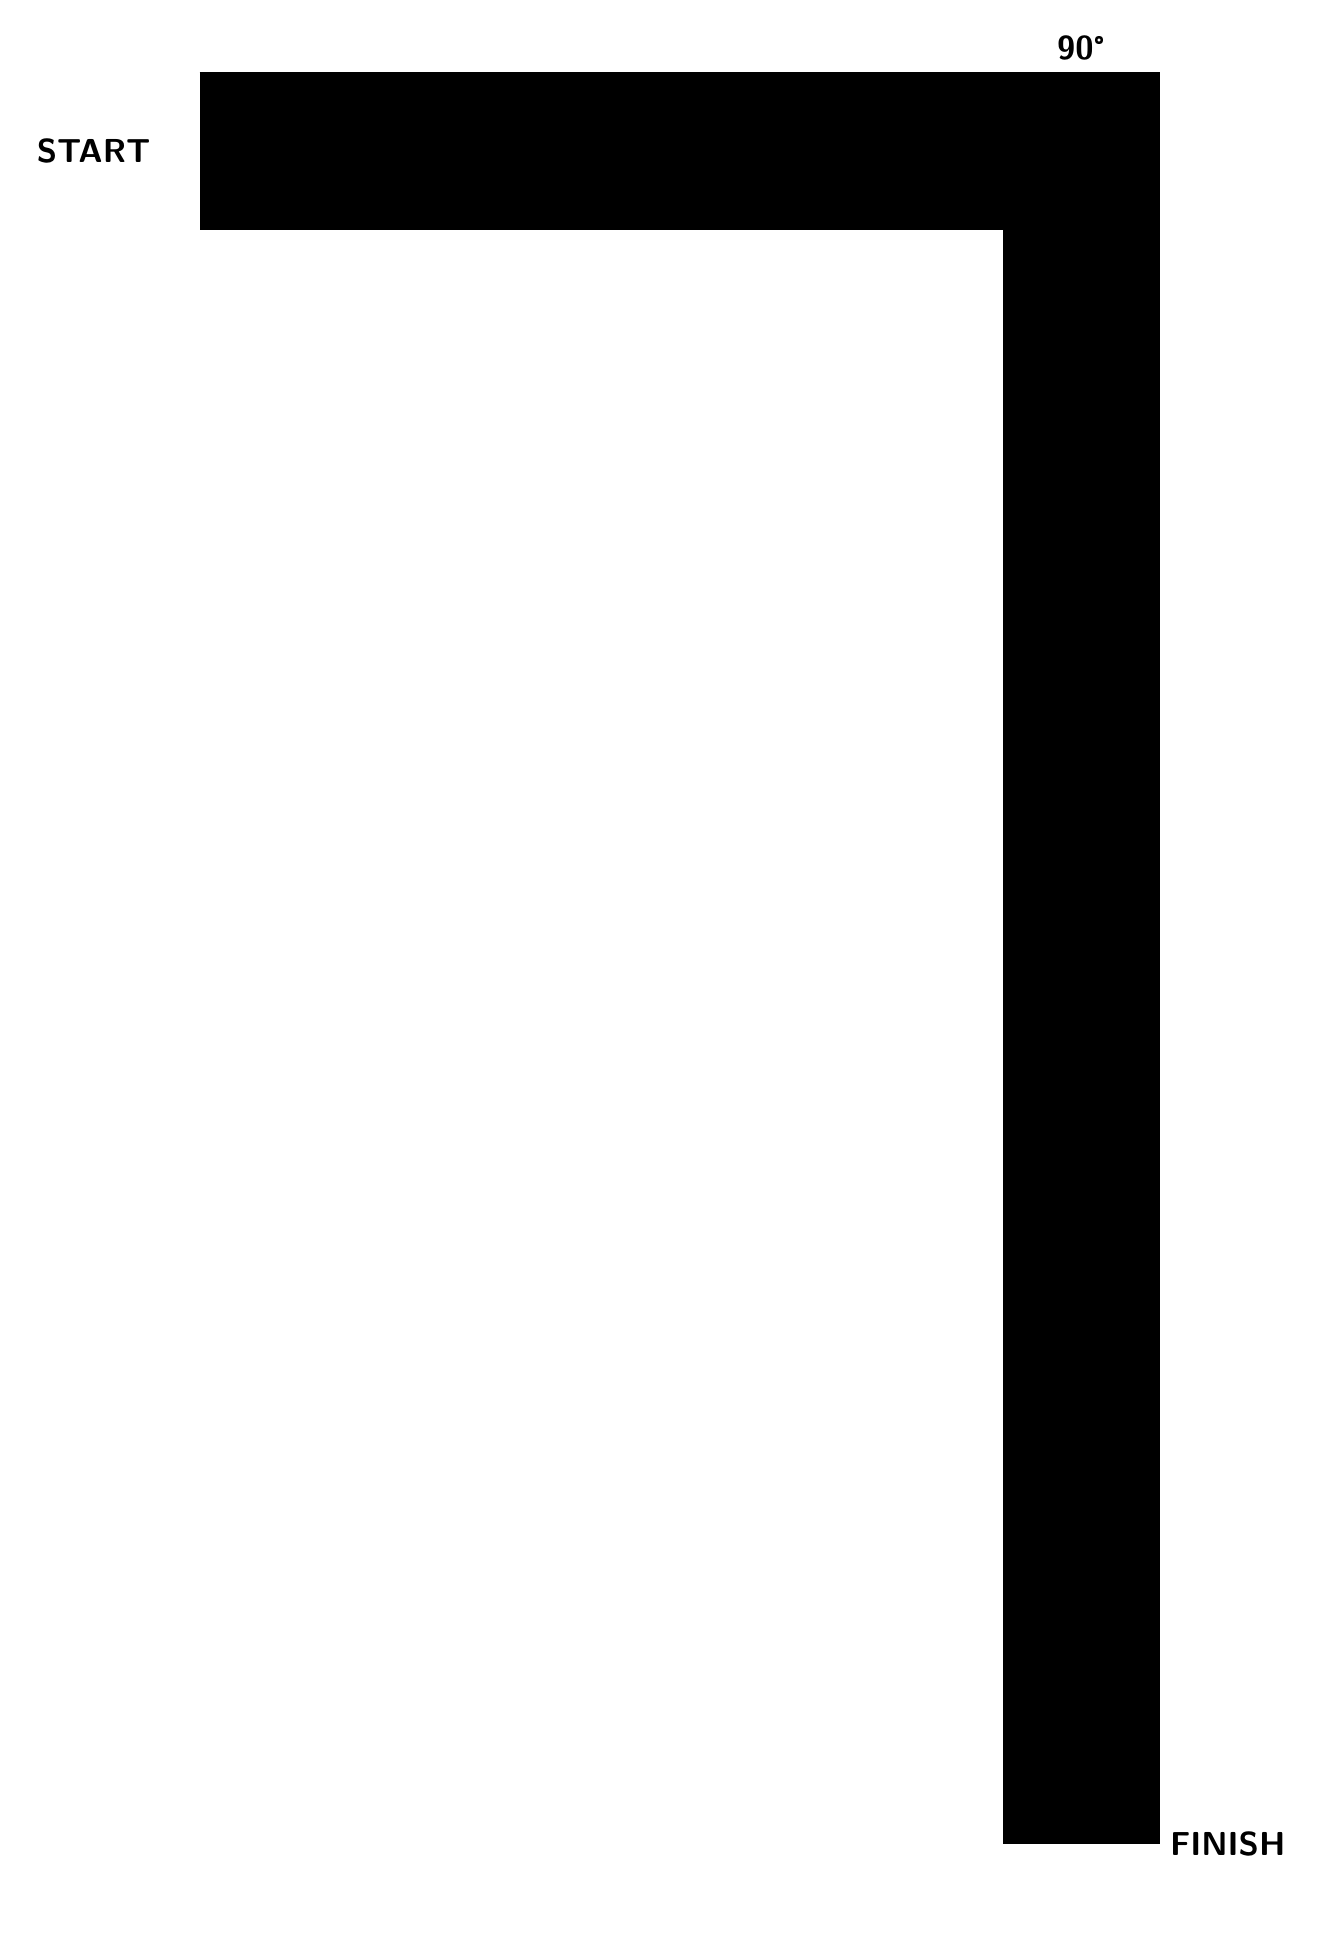
\begin{tikzpicture}[x=1mm,y=1mm]
    \draw[line width=20mm, black, line cap=butt] (18,245) -- (130,245) -- (130,30);
    \node[anchor=east, font=\large\bfseries] at (13,245) {START};
    \node[anchor=west, font=\large\bfseries] at (140,30) {FINISH};
    \node[font=\large\bfseries] at (130,258) {90\textdegree};
  \end{tikzpicture}
\end{center}
\end{document}
